\documentclass[10pt]{article}
\usepackage[utf8]{inputenc}
\usepackage[spanish]{babel}
\usepackage{amsmath}
\usepackage{amsfonts}
\usepackage{amssymb}
\usepackage{graphics}
\usepackage{graphicx}
\usepackage[left=2cm,right=2cm,top=2cm,bottom=2cm]{geometry}
\usepackage{imakeidx}
\makeindex[columns=3, title=Alphabetical Index, intoc]
\usepackage{listings}
\usepackage{xcolor}
\usepackage{multicol}
\usepackage{changepage}
\usepackage{float}
\usepackage{cite}
\usepackage{url}
\usepackage{hyperref}
\usepackage[document]{ragged2e}
\hypersetup{
    colorlinks=true,
    linkcolor=blue,
    filecolor=magenta,
    urlcolor=blue,
}

\definecolor{codegreen}{rgb}{0,0.6,0}
\definecolor{codegray}{rgb}{0.5,0.5,0.5}
\definecolor{codepurple}{rgb}{0.58,0,0.82}
\definecolor{backcolour}{rgb}{0.95,0.95,0.92}

\lstdefinestyle{mystyle}{
    backgroundcolor=\color{backcolour},
    commentstyle=\color{codegreen},
    keywordstyle=\color{magenta},
    numberstyle=\tiny\color{codegray},
    stringstyle=\color{codepurple},
    basicstyle=\ttfamily\footnotesize,
    breakatwhitespace=false,
    breaklines=true,
    captionpos=b,
    keepspaces=true,
    numbers=left,
    numbersep=5pt,
    showspaces=false,
    showstringspaces=false,
    showtabs=false,
    tabsize=3
}

\lstset{style=mystyle}

\title{Centro de Investigación en Cómputo\\Instituto Politécnico Nacional\\Metaheurísticas\\Actividad No. 8\\ Solución de problemas mediante Recocido Simulado\\Curso impartido por: Dra Yenny Villuendas Rey}

\author{Adrian González Pardo}

\date{\today}

\newcommand\tab[1][1cm]{\hspace*{#1}}

\begin{document}
\maketitle
\section{Recocido Simulado (Simulated Annealing, SA)}
\begin{center}
  \begin{tabular}{|p{6cm}|p{6cm}|}
    \hline
    Ventajas & Desventajas \\
    \hline
    Permite obtener una solución aproximada al mínimo global & Puede llegar a pasar que en la siguiente iteración a la solución salga del mínimo global y este se alcance un resultado mínimo local \\
    \hline
    Permite encontrar soluciones razonables (En tiempo) & La solución encontrada puede no ser la mejor\\
    \hline
    Utiliza poca memoria & No permite vuelta atras en más de 1 paso\\
    \hline
  \end{tabular}
\end{center}
\section{Pseudocódigo SA}
\lstinputlisting[language=Ruby]{./pseudo.rb}
\section{SA vs RMHC}
La diferencia más notable entre estos dos algoritmos, es notablemente que el RMHC se basa en la mutación aleatoria de un conjunto de datos, generando un camino de solución del arbol de soluciones, mientras que SA parte de una solución donde el mismo algoritmo esta bioinspirado en un proceso físico que busca un ablandamiento para la formación o moldeo de estructuras de metal, entonces si bien ambos son algoritmos heurísticos RMHC se aplica en problemas cuya solución puede ser mutada y en este caso no puede salir de un mínimo local si este cae en ese espacio, mientras que SA permite admitir una respuesta no optima para seguir explorando el espacio de soluciones.
\section{Algoritmo de búsqueda de vecinos adaptativa}
En el paper podemos observar el algoritmo metaheurístico, en el cual su área de solución es en un espacio de dominio discreto, pero el autor nos hace mención con respecto a hacer una hibridación del problema usando un dominio continuo, en el cual se permite la idea de hacer un uso de algoritmo donde dependiendo la obtención del valor se decide por usar el dominio discreto o el dominio continuo para con este se pueda dar idea a la traslación y rotación del objeto que mencionan en el paper, para así no desperdiciar regiones de área que puden ser utilizadas para acomodar $P_{i}$ objetos.

\section{Investigación de los ultimos 3 años aplicando el algoritmo de SA}
\begin{enumerate}
  \item Agosto de 2020. Diseño del controlador de regulación automática de voltaje usando SA hibrido con algoritmos de optimización de Forrajeo de mantarraya. \underline{\href{https://www.sciencedirect.com/science/article/pii/S2090447920301416}{Paper}}
  \item Enero de 2020. Una nueva técnica híbrida de programación genética basada en SA para predecir la capacidad de carga máxima de las pilas. \underline{\href{https://link.springer.com/article/10.1007/s00366-019-00932-9}{Paper}}
  \item Junio de 2018. Optimización de SA evolutivo multiobjetivo para el equilibrado de la línea de desmontaje multirrobótico de modelo mixto con tiempo de procesamiento de intervalo. \underline{\href{https://www.tandfonline.com/doi/abs/10.1080/00207543.2019.1602290}{Paper}}
\end{enumerate}
\section{Aplicaciones SA}
\subsection{Knapsack}
Modelación Matemática\\
Sean dos funciones
\[f(x)=\sum_{i=1}^{N}x^{'}_{i}h(x_{i})\]
\[g(x)=\sum_{i=1}^{N}x^{'}_{i}p(x_{i})\;<=\;peso\_maximo\]
Donde:\\
\(\displaystyle X\;es\;un\;vector\;de\;la\;forma\;X=[x_{1},x_{2},\cdots,x_{N}]\)\\\vspace{0.25cm}
\(\displaystyle X^{'}\;es\;un\;vector\;el\;cual\;es\;parecido\;a\;X\;pero\;sus\;valores\;x_{i}^{'}\in[0,1]\;y\;x_{i}^{'}\in\mathbb{Z}\)\\\vspace{0.25cm}
\(\displaystyle h(x)\;es\;una\;funci\acute{o}n\;la\;cual\;devuelve\;el\;beneficio\;total\;de\;los\;objetos\;x_{i}\;en\;la\;mochila\)\\\vspace{0.25cm}
\(\displaystyle p(x)\;es\;una\;funci\acute{o}n\;la\;cual\;devuelve\;el\;peso\;total\;de\;los\;objetos\;x_{i}\;en\;la\;mochila\)\\\vspace{0.25cm}
En el cual el algoritmo de SA busca iterar sobre cada contenido o casilla del vector $X^{'}$ de tal forma que se obtiene una solución y sobre esta se busca encontrar una mejor solución.\\
Por lo cual el test objetivo del algoritmo es encontrar el optimo global sin que este pueda caer en el optimo local o en otra zona.\\
En el algoritmo se creara conjunto $S$ cuya evaluación es una solución aleatoria al problema, en el cual al interactuar con el algoritmo SA se generara un conjunto $S^{'}$ el cual sera retornado como una mejor solución a $S$\\\vspace{0.5cm}
\textbf{Estructura propuesta para su solución:}\\
Si bien en este problema podemos resolverso en un lenguaje de alto nivel podemos hacer uso de un arreglo dinámico en el cual podamos añadir elementos cuyos atributos son los siguientes:\\
\begin{itemize}
  \item Costo: Valor entero o valor real
  \item Beneficio: Valor entero o valor real
  \item Selección: Valor booleano
\end{itemize}
De modo que a traves de este arreglo se pueda realizar la operación producto para la obtención del costo total y la obtención del peso total.

\subsection{Travel Salesman Problem TSP}
Modelación Matemática\\
Sea la función
\[f(x)=\sum_{i=1,j=1}^{N,N}x^{'}_{i,j}g(x_{i,j})\]
Donde:\\
\(\displaystyle X\;es\;una\;matriz\;de\;NxN\;la\;cual\;trabajara\;para\;obtener\;el\;costo\;con\;la\;funci\acute{o}n\;g(x)\)\\\vspace{0.25cm}
\(\displaystyle X^{'}\;es\;una\;matriz\;de\;NxN\;la\;cual\;contiene\;valores\;que\;permiten\;saber\;si\;el\;nodo\;es\;considerado\;o\;no\;para\;la\;soluci\acute{o}n\;\)\\\vspace{0.25cm}
\(\displaystyle La\;notaci\acute{o}n\;(i,j)\;significa\;\;i\;como\;nodo\;origen\;que\;va\;a\;j\)\\\vspace{0.25cm}
\(\displaystyle x^{'}_{i,j}\;es\;un\;valor\;de\;la\;matriz,\;donde\;x^{'}_{i,j}\in[0,1]\;y\;x_{i,j}\in\mathbb{Z}\)\\\vspace{0.25cm}
\(\displaystyle Si\;x_{i,j}=-1\;significa\;que\;no\;hay\;una\;conexi\acute{o}n\;de\;i\;a\;j\)\\\vspace{0.25cm}
\(\displaystyle g(x)\;es\;una\;funci\acute{o}n\;la\;cual\;devuelve\;el\;valor\;costo\;de\;ir\;de\;i\;a\;j\)\\\vspace{0.25cm}
De tal forma que este algoritmo de SA busca iterar sobre el contenido de una solución cualquiera y sobre cada vertice que este modifique el algoritmo buscara realizar una operación de intercambio de la forma $x_{i,j}$ cambia con $x_{j,i}$ de tal forma que el movimiento sea valido y este modifique la solución.\\
El test objetivo de esta solucion es encontrar una solución de minimización de costo de tal forma que la solución recorra todos los nodos.\\
Finalmente el valor inicial del algoritmo es una matriz $S$ cuyos valores realizaran el producto sobre su semenjante $S^{'}$ en el cual podran conocerse el costo inicial de la solución, al entrar al algoritmo de SA obtendremos una matriz que operara sobre $S^{'}$ y modificara los valores del camino tomado y de forma teorica se obtendra una matriz $T^{'}$ la cual al interactuar con el producto de $S$ es mejor que $S^{'}$.\vspace{0.5cm}

\textbf{Estructura propuesta para la solución:}\\
Para este problema podemos hacer uso de una estructura arreglo dinámico en el cual tendre los siguientes atributos arreglo de costos para cambiar al siguiente vertice, el arreglo de selección booleano que permitira conocer si el camino es tomado. Ahora bien ese arreglo dinámico dependiendo de la entrada de vertices podemos evolucionarlo a una estructura bicola circular en el caso de que sea un grafo completo es decir que todos sus vertices estan conectados entre si, de modo que al obtener una solución $S$ este pueda rotar los indices formando una solución $S^{'}$.



\subsection{Función de Minimización en D dimensiones}
Modelación Matemática\\
Sea la función
\[f(x)=\sum_{i=1}^{N}x_{i}^{2}\]
Donde:\\
\(\displaystyle x_{i}\in\mathbb{R}\)\\\vspace{0.25cm}Descrito en los intervalos \(\displaystyle x_{i}\in[-10,10]\)\\\vspace{0.25cm}
Donde sabemos que los puntos mínimos de cada $x_{i}$ los encontramos cuando el valor asignado a el es $x_{i}=0$ por lo tanto el ir variando los valores para que el programa se acerque hacia $0$\\
De tal manera que el algoritmo de SA seleccionara 1 indice en el cual se le asignara un valor a $x_{i}$.\\
En el test objetivo es encontrar 1 punto aproximado en el que la función se aproxime a $0$ o en el que al menos una coordenada $x_{i}\sim 0$
\\
En ello generaremos un conjunto solución $S$ el cual contendra los puntos $x_{i}$ de modo que al ser evaluado en la función matemática obtendremos un valor $Y$ que sera el costo total de evaluar ese punto y considerarlo punto mínimo, una vez pasando por el algorimto SA obtendremos un valor $S^{'}$ en el cual al pasar por la función a evaluar se obtendra un $Y^{'}$ de modo que teóricamente al comparar dichos valores obtenidos $Y^{'}$ es mejor y por lo tanto $S^{'}$ es un mejor punto mínimo de la función.\vspace{0.5cm}
\\\textbf{Estructura propuesta para la solución:}\\
Para este problema podemos pensar en un vector o arreglo dinámico de $D$ dimensiones en el cual evalualeremos por la función matemática que nos arrojara la suma de los cuadrados de cada punto $x_i$ de modo que podremos trabajar sobre la misma para obtener un mínimo mejor evaluado que otro.
\clearpage
\section{Implementación y ejecución}
\subsection{Knapsack}
La interfaz por línea de comandos es la siguiente para el programa:
\begin{center}
  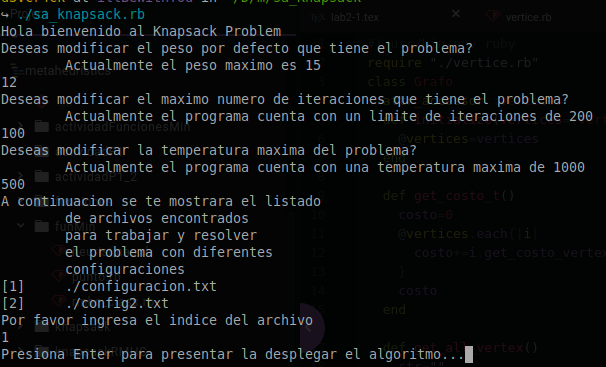
\includegraphics[scale=0.5]{imgs/int-knap.png}
  \\\textit{Figura 1: Interfaz del problema Knapsack en el cual se puede modificar máximo de iteraciones, temperatura máxima, peso máximo de la mochila, y el archivo de configuraciones}
\end{center}
La ejecución del problema arrojo los siguientes resultados de dos corridas:
\begin{center}
  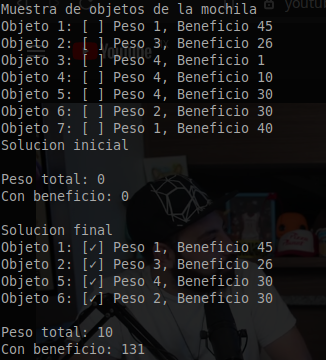
\includegraphics[scale=0.5]{imgs/k_sol-1.png}\\
  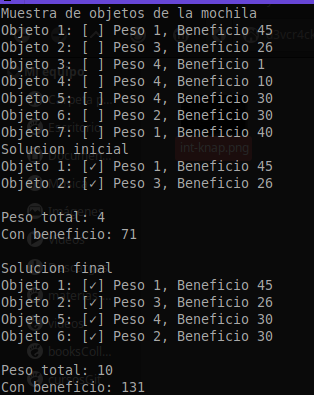
\includegraphics[scale=0.5]{imgs/k_sol-2.png}
\end{center}
\subsection{TSP}
La configuración del grafo es:
\begin{center}
  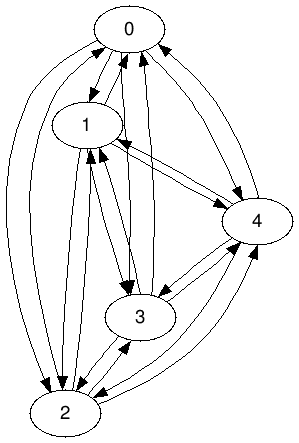
\includegraphics[scale=0.5]{imgs/grafo.png}
\end{center}
La interfaz por línea de comandos es la siguiente:
\begin{center}
  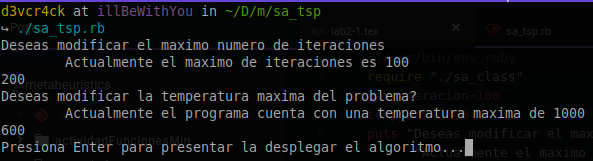
\includegraphics[scale=0.5]{imgs/int-tsp.png}\\
  \textit{Figura 2: Interfaz del TSP en cual se puede modificar el máximo de iteraciones, y temperatura máxima, destacando que la implementación se busca la solución a una entrada de un grafo completo, es decir 1 vertice apunta a los demas de igual forma.}
\end{center}
La ejecución arrojo los siguientes resultados de la configuración:
\begin{center}
  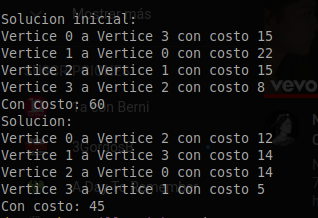
\includegraphics[scale=0.5]{imgs/tsp_sol-1.png}\\
  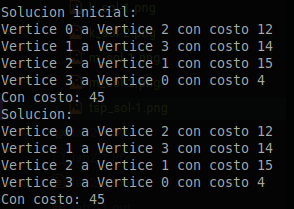
\includegraphics[scale=0.5]{imgs/tsp_sol-2.png}
\end{center}
\subsection{Función mínimos}
La interfaz por línea de comandos es la siguiente:
\begin{center}
  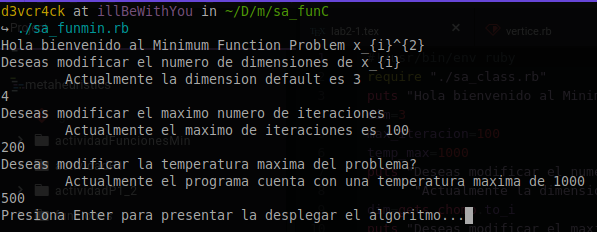
\includegraphics[scale=0.5]{imgs/int-min.png}
  \\\textit{Figura 3: Interfaz del problema de la función \(\displaystyle f(x)=\sum_{i=1}^{D}x_{i}^{2}\) en el cual se puede modificar máximo de iteraciones, temperatura máxima y número de dimensiones de la función}
\end{center}
La ejecución arrojo los siguientes resultados:
\begin{center}
  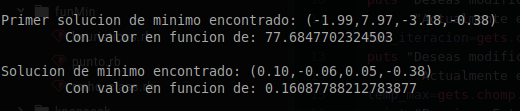
\includegraphics[scale=0.5]{imgs/m_sol-1.png}\\
  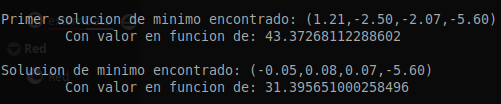
\includegraphics[scale=0.5]{imgs/m_sol-2.png}
\end{center}


\end{document}
